\documentclass[aspectratio=169,usenames,dvipsnames]{beamer}
\usetheme{metropolis}
%\usecolortheme[snowy,cautious]{owl}
\usecolortheme[snowy]{owl}
\metroset{block=fill}

% For regular math font
\usefonttheme[onlymath]{serif}

\usepackage{appendixnumberbeamer}
\usepackage{booktabs}
\usepackage{fancyvrb}
\usepackage{makecell}
\usepackage{xcolor}
%\usepackage{soul}
\usepackage[normalem]{ulem}
\usepackage{hyperref}
\usepackage{siunitx}
\usepackage{amsmath}
\usepackage{amssymb}
\usepackage{color}
\usepackage{listings}
\usepackage[normalem]{ulem}
\hypersetup{colorlinks,allcolors=.,urlcolor=blue}

% Not used
\definecolor{mygreen}{rgb}{0,0.6,0}
\definecolor{mygray}{rgb}{0.5,0.5,0.5}
\definecolor{mymauve}{rgb}{0.58,0,0.82}
\definecolor{myblue}{rgb}{0,0,1}
% For C
\definecolor{comment}{RGB}{0,128,0} % dark green
\definecolor{string}{RGB}{255,0,0}  % red
\definecolor{keyword}{RGB}{0,0,255} % blue

% Fix dashs/hyphens in listings
\makeatletter
\lst@CCPutMacro\lst@ProcessOther {"2D}{\lst@ttfamily{-{}}{-{}}}
\@empty\z@\@empty
\makeatother

\newfontfamily\Bera{Bitstream Vera Sans Mono}[Scale=1]
\newfontfamily\TgCursor{TeX Gyre Cursor}[Scale=1]
\newfontfamily\Dejavu{DejaVu Sans Mono}[Scale=1]
%\newfontfamily\Consolas{Consolas}[Scale=0.85]
\newfontfamily\Consolas{Consolas}[Scale=1]

\lstdefinestyle{global} {
%  basicstyle=\fontfamily{cmvtt}\selectfont
%  basicstyle=\tiny\ttfamily,
%  basicstyle=\tiny\Dejavu,
  basicstyle=\tiny\Consolas,
  backgroundcolor=\color{white},
  commentstyle=\itshape\color{comment},
  stringstyle=\color{string},
  keywordstyle=\bfseries\color{keyword},
  %identifierstyle=\bfseries,
  numbers=left,
  numberstyle=\tiny,
  numbersep=5pt,
  frame=lines,
  breaklines=true,
  prebreak=\raisebox{0ex}[0ex][0ex]{\ensuremath{\hookleftarrow}},
  showstringspaces=false,
  upquote=true,
  tabsize=8,
  escapeinside=\`\`,
}

\lstdefinestyle{c} {
  escapeinside=\`\`,
  morekeywords={u8,u16,u32,s8,s16,s32,size_t, ssize_t},
}

\lstdefinestyle{make} {
  language=make,
  morekeywords={if,ifneq,else,elseif,endif},
}

\lstset {
  language=C,
  style=global,
}

% allowframebreaks numbering in the title
\newcounter{cont}
\makeatletter
\setbeamertemplate{frametitle continuation}{%
    \setcounter{cont}{\beamer@endpageofframe}%
    \addtocounter{cont}{1}%
    \addtocounter{cont}{-\beamer@startpageofframe}%
    (\insertcontinuationcount/\arabic{cont})%
}
\makeatother

\title{Kernel Course: Lecture 18}
\subtitle{Working with Embedded Buses}
\date{\today}
\author{Sam Protsenko}
\institute{GlobalLogic}

\begin{document}

\sisetup{
  math-rm = \mathrm,
  inter-unit-product = \ensuremath{{}\cdot{}},
  per-mode = fraction,
%  fraction-function = \tfrac,
%  unit-color = purple
}

\maketitle

\begin{frame}{Agenda}
  \setbeamertemplate{section in toc}[sections numbered]
  \tableofcontents[hideallsubsections]
\end{frame}

% ------------------------------------------------------------------------------

\section{I2C Overview}

\subsection{Embedded Buses Overview}

\begin{frame}
  \frametitle{Serial vs Parallel}
  \begin{columns}
    \column{0.6\textwidth}
      \begin{figure}
        \centering
        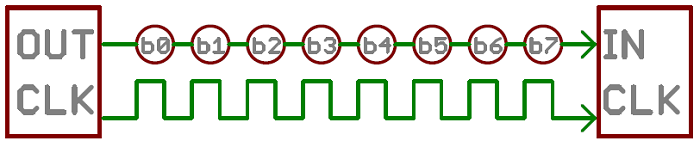
\includegraphics[scale=0.45]{images/serial-bus.png}
        \caption{Serial Bus}
      \end{figure}
      Serial buses have won:
      \begin{itemize}
        \item[] \textcolor{green}{(+)} Easier to implement the HW
        \item[] \textcolor{green}{(+)} Can be used on higher frequencies
      \end{itemize}
      Parallel buses are used for in-chip communications
    \column{0.4\textwidth}
      \begin{figure}
        \centering
        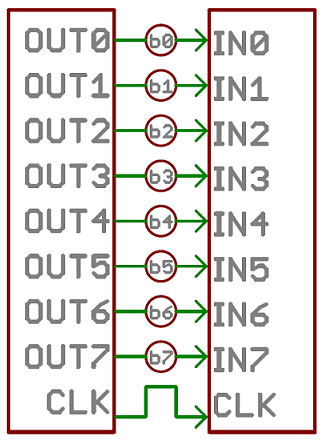
\includegraphics[scale=0.45]{images/parallel-bus.png}
        \caption{Parallel Bus}
      \end{figure}
  \end{columns}
\end{frame}

\begin{frame}
  \frametitle{Serial Bus: Async vs Sync}
  \begin{columns}
    \column{0.45\textwidth}
      \begin{figure}
        \centering
        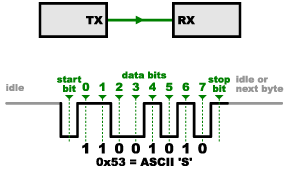
\includegraphics[scale=0.69]{images/serial-async.png}
        \caption{Asynchronous}
      \end{figure}
    \column{0.55\textwidth}
      \begin{figure}
        \centering
        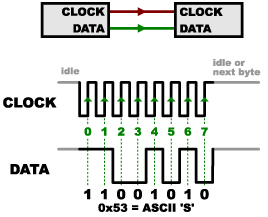
\includegraphics[scale=0.69]{images/serial-sync.png}
        \caption{Synchronous}
      \end{figure}
  \end{columns}
  \begin{columns}
    \column{0.45\textwidth}
      \begin{itemize}
        \item[] \alert{(-)} Low-speed transmission
        \item[] \textcolor{green}{(+)} Long distance
      \end{itemize}
    \column{0.55\textwidth}
      \begin{itemize}
        \item[] \textcolor{green}{(+)} High-speed transmission
        \item[] \alert{(-)} Short distance (due to clock skew)
      \end{itemize}
  \end{columns}
\end{frame}

\begin{frame}
  \frametitle{Buses on Embedded Boards}
  \begin{itemize}
    \item Serial buses:
      \begin{itemize}
        \item SPI
        \item \textbf{I2C / SMBus}
        \item UART
        \item USB
        \item 1-wire
        \item CAN
        \item PCI-e
      \end{itemize}
    \item Parallel buses (rarely used in Embedded):
      \begin{itemize}
        \item ISA
        \item PCI
        \item Parallel port
      \end{itemize}
  \end{itemize}
\end{frame}

\begin{frame}
  \frametitle{Discoverable vs Non-discoverable}
  \begin{columns}
    \column{0.5\textwidth}
      \begin{block}{Discoverability}
      \alert{Discoverable bus} is able to find connected devices during
      \textit{enumeration}, so that no device tree entry is needed.
      \end{block}
      \begin{itemize}
        \item Discoverable buses:
          \begin{itemize}
            \item USB
            \item PCI
          \end{itemize}
        \item Non-/semi-discoverable buses:
          \begin{itemize}
            \item SPI
            \item \textbf{I2C}
            \item Platform devices (pseudo-bus)
          \end{itemize}
      \end{itemize}
    \column{0.5\textwidth}
      \begin{figure}
        \centering
        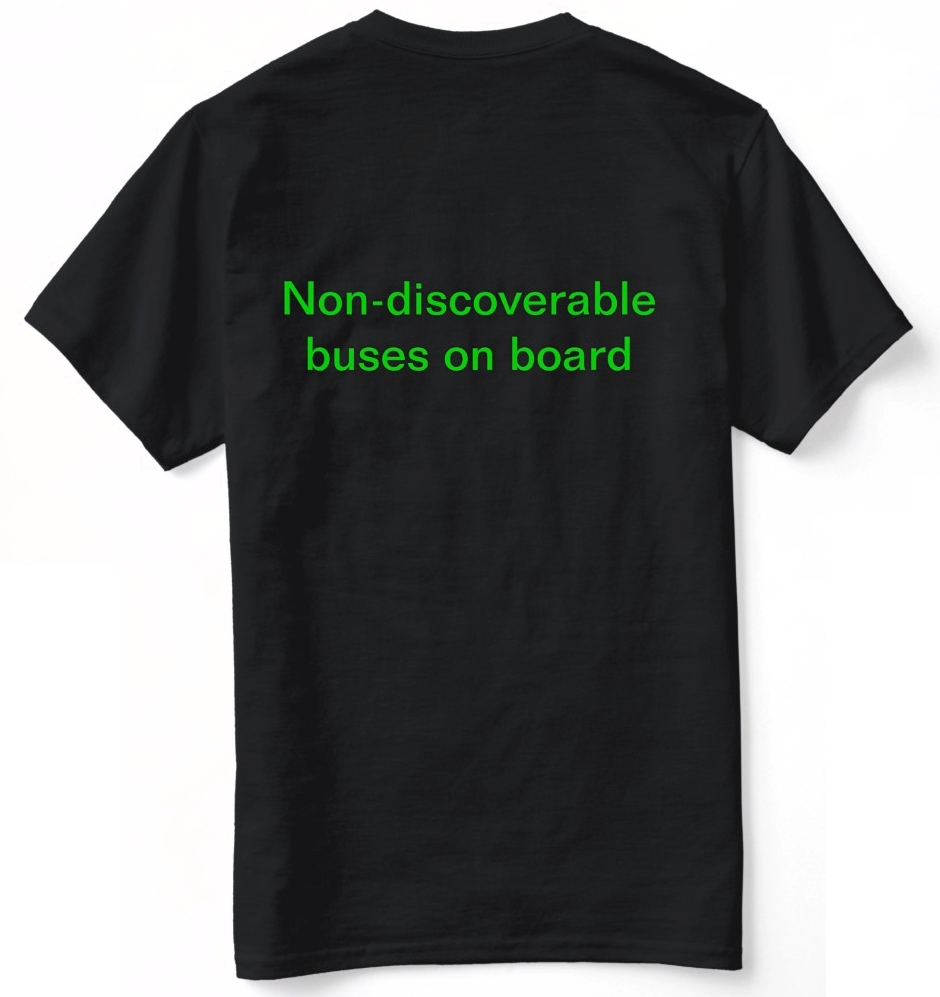
\includegraphics[scale=0.25]{images/t-shirt.png}
      \end{figure}
      \vspace*{-6mm}
  \end{columns}
\end{frame}

% ------------------------------------------------------------------------------

\subsection{I2C Bus Overview}

\begin{frame}
  \frametitle{I2C Basic Facts}
  \begin{itemize}
    \item Low-speed bus to connect on-board and external devices to SoC
    \item Only two wires (clock, data)
    \item Allows several devices on one bus
    \item Devices have I2C addresses
    \item Master/slave
    \item Master initiates communication and provides clock signal
    \item Multi-master scheme is allowed
    \item Keep wires short (up to \SI{0.5}{\m} @ \SI{400}{\kilo\Hz})
  \end{itemize}
\end{frame}

\begin{frame}
  \frametitle{Usual I2C Devices}
  \begin{itemize}
    \item Sensors (temp, accel, magn, gyro, ...)
    \item Real-Time Clock (RTC)
    \item EEPROM
    \item I/O Expanders
    \item LCD Displays
    \item Touch screens
    \item ...a lot more, wherever low-speed bus is OK
  \end{itemize}
\end{frame}

\begin{frame}
  \frametitle{I2C Bus Example}
  \begin{figure}
    \centering
    \includegraphics[scale=0.35]{images/i2c-bus.pdf}
    \caption{Client Devices on I2C Bus}
  \end{figure}
\end{frame}

% ------------------------------------------------------------------------------

\subsection{I2C Protocol Overview}

\begin{frame}
  \frametitle{I2C Connection}
  \begin{figure}
    \centering
    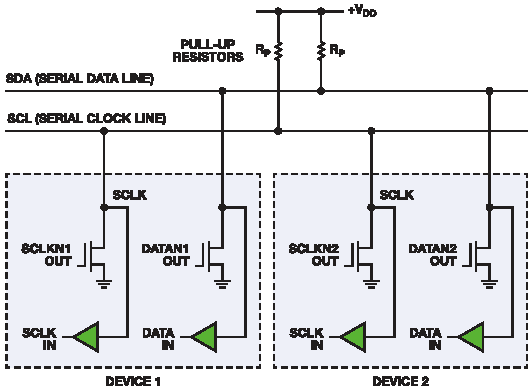
\includegraphics[scale=0.9]{images/i2c-connection.pdf}
    \caption{Scheme of Regular I2C Connection}
  \end{figure}
  \vspace*{-10mm}
\end{frame}

\begin{frame}
  \frametitle{Open Drain}
  \begin{figure}
    \centering
    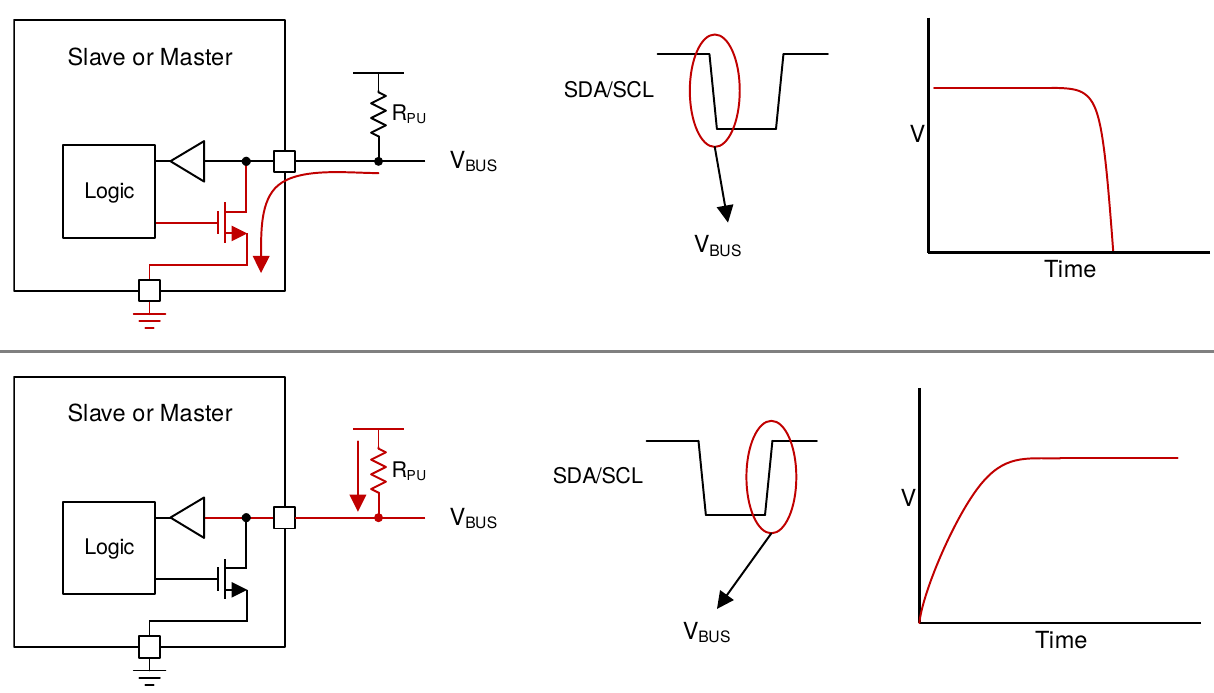
\includegraphics[scale=0.3]{images/open-drain.png}
    \caption{Open Drain Function in I2C Connection}
  \end{figure}
  \vspace*{-10mm}
\end{frame}

\begin{frame}
  \frametitle{I2C Packet}
  \begin{figure}
    \hspace*{-8mm}
    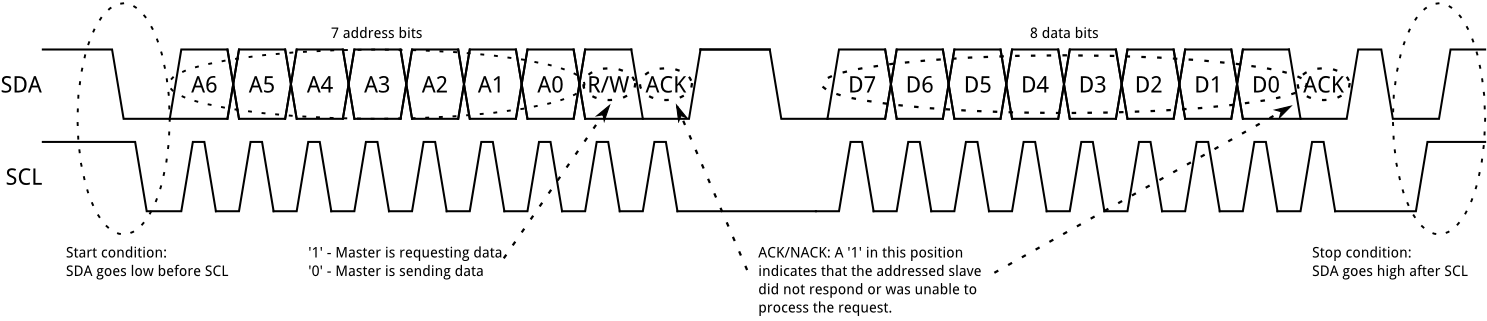
\includegraphics[scale=0.58]{images/i2c-packet.png}\hspace*{-8mm}
    \caption{I2C Packet Format}
  \end{figure}
\end{frame}

\begin{frame}
  \frametitle{I2C Packet: Write Register}
  \begin{figure}
    \hspace*{-8mm}
    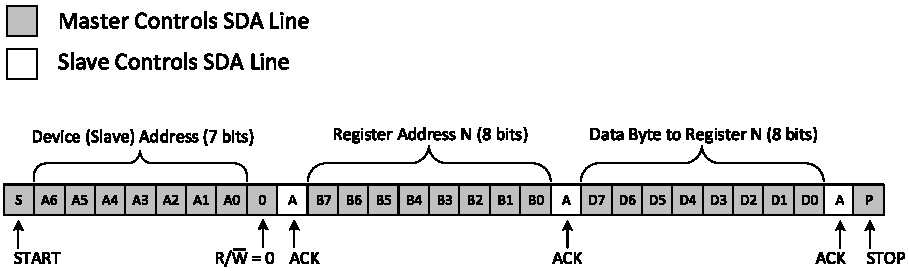
\includegraphics[scale=0.9]{images/i2c-write-reg.pdf}\hspace*{-8mm}
    \caption{I2C Write to Slave Device's Register}
  \end{figure}
\end{frame}

\begin{frame}
  \frametitle{I2C Packet: Read Register}
  \begin{figure}
    \hspace*{-10mm}
    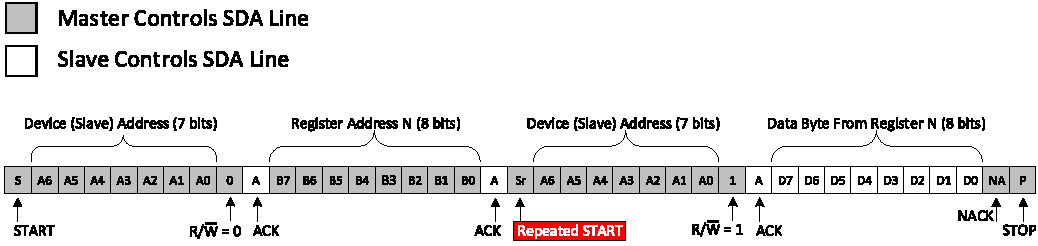
\includegraphics[scale=0.9]{images/i2c-read-reg.pdf}\hspace*{-10mm}
    \caption{I2C Read from Slave Device's Register}
  \end{figure}
\end{frame}

% ------------------------------------------------------------------------------

\section{RTC Module}

\begin{frame}
  \frametitle{TinyRTC Module Schematic}
  \begin{figure}
    \centering
    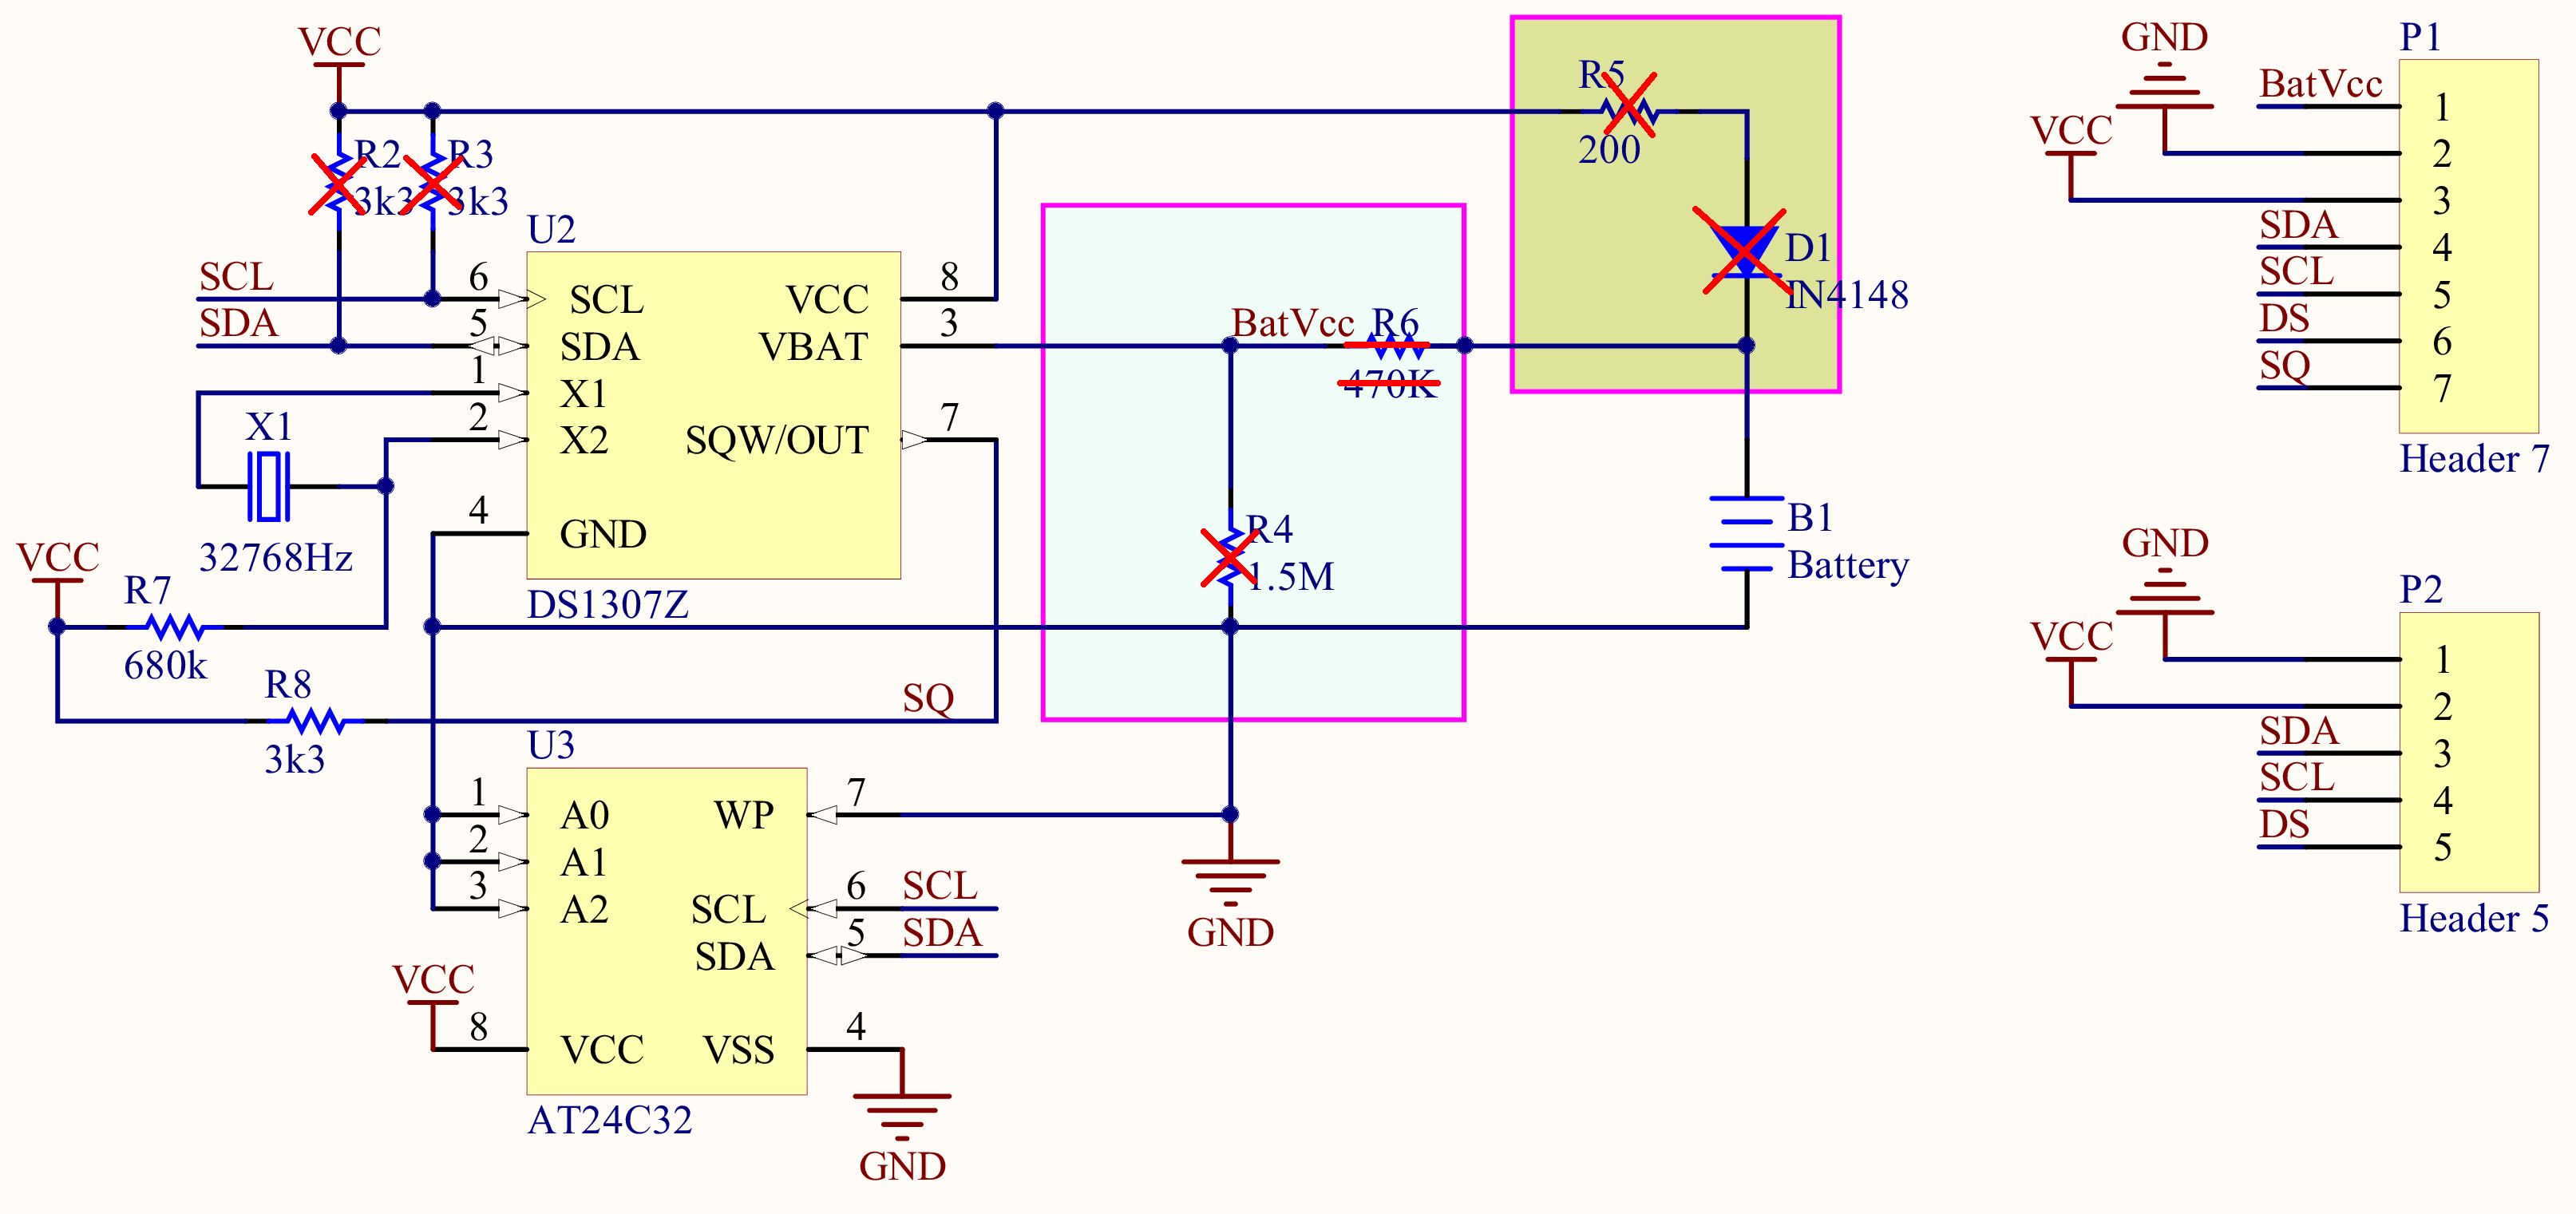
\includegraphics[scale=0.15]{images/tinyrtc-scheme-mod.png}
  \end{figure}
  \vspace*{-12mm}
\end{frame}

\begin{frame}
  \frametitle{TinyRTC Module Changes}
  \begin{itemize}
    \item Remove module's I2C pull-up resistors (R2, R3)
    \begin{itemize}
      \item VCC = 5V in module
      \item BBB I2C voltage for ``1'' is 3.3V
      \item \alert{We'll use internal pull-ups to 3.3V for I2C lines}
    \end{itemize}
    \item Remove charging scheme (R5, D1)
    \begin{itemize}
      \item Modules have non-rechargeable batteries (CR2032) by mistake
            (should have recharegeabe LIR2032 instead)
      \item Also remove divider (R4, R6); connect battery directly to VBAT
            instead
    \end{itemize}
    \item Crystal X1 is soldered to GND, to improve stability
    \item Soldered pin header sockets, to ease the prototyping
  \end{itemize}
\end{frame}

\begin{frame}
  \frametitle{TinyRTC Module Connection}
  \begin{figure}
    \centering
    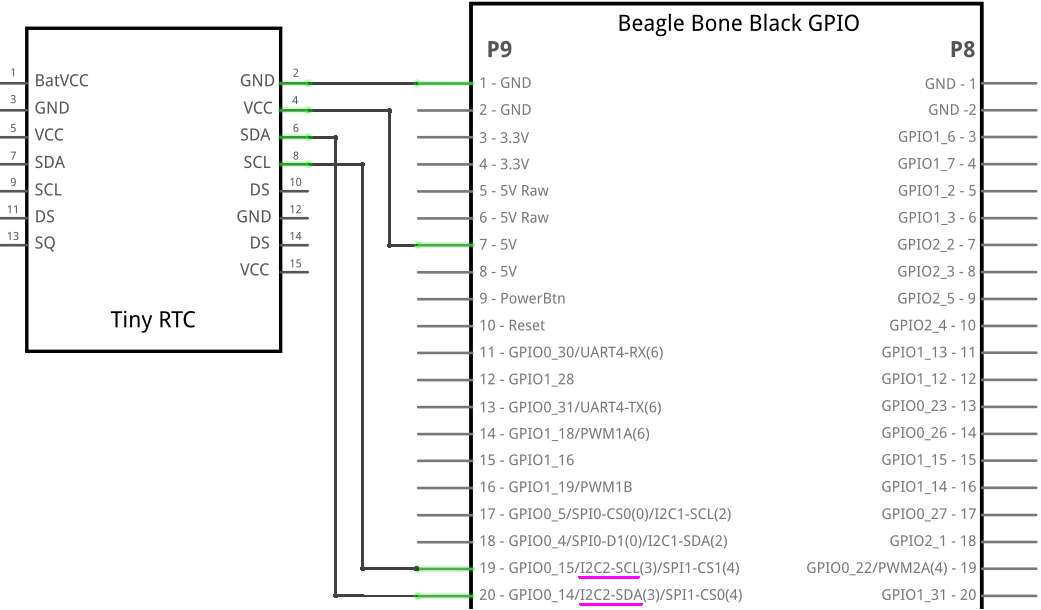
\includegraphics[scale=1]{images/bbb-rtc_schem.png}
  \end{figure}
  \vspace*{-12mm}
\end{frame}

\begin{frame}
  \frametitle{TinyRTC Module Connection (cont'd)}
  \begin{figure}
    \centering
    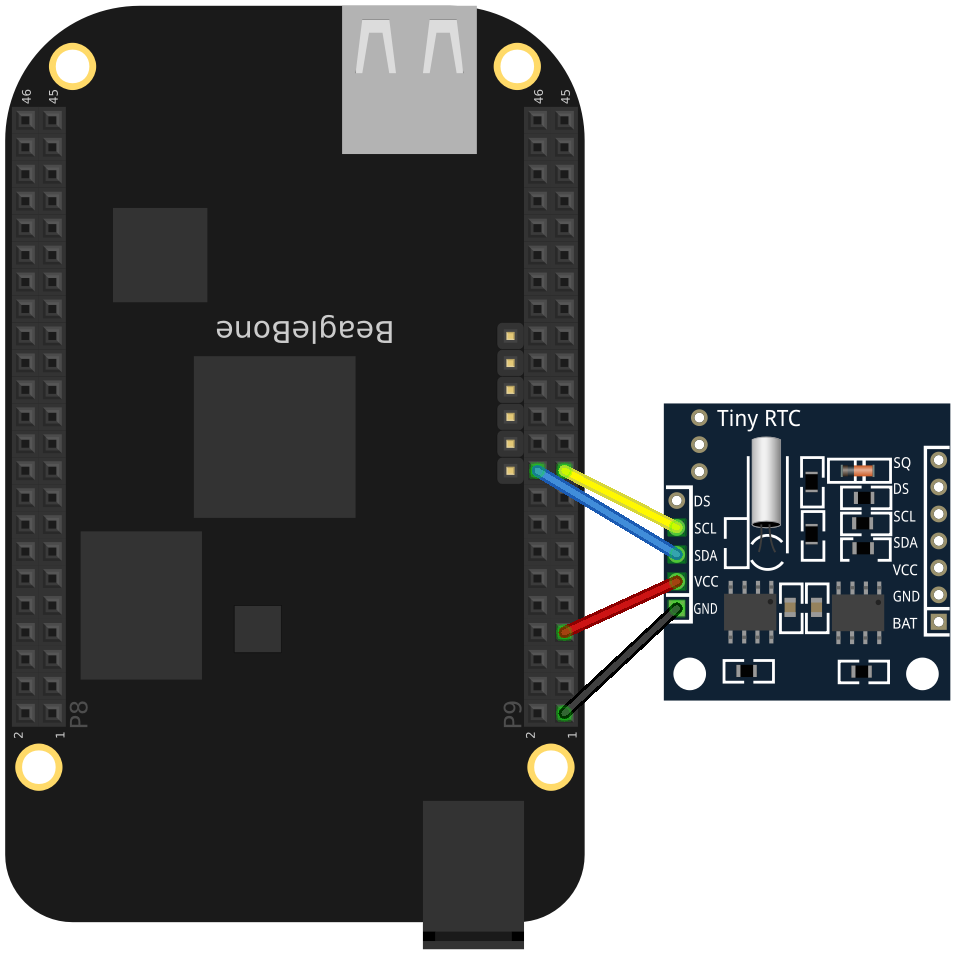
\includegraphics[scale=0.7]{images/bbb-rtc_bb.png}
  \end{figure}
  \vspace*{-12mm}
\end{frame}

\begin{frame}
  \frametitle{RTC Read/Write}
  \vspace*{-2mm}
  \begin{figure}
    \centering
    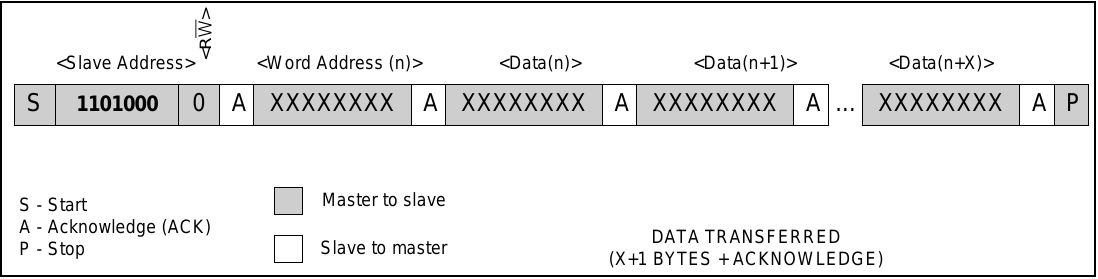
\includegraphics[scale=0.35]{images/ds1307-write.png}
    \caption{DS1307 Data Write}
  \end{figure}
  \vspace*{-5mm}
  \begin{figure}
    \centering
    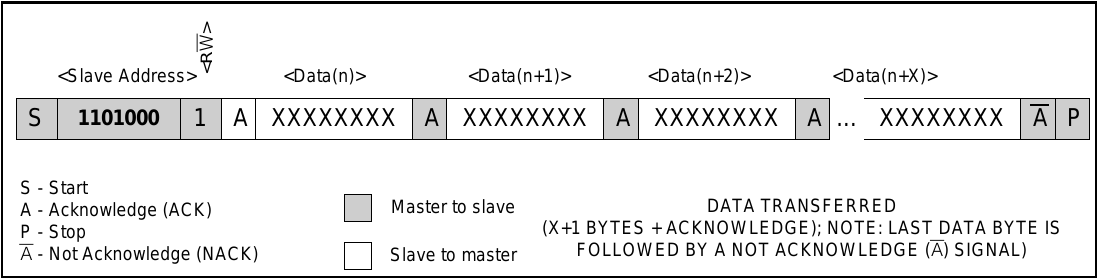
\includegraphics[scale=0.35]{images/ds1307-read.png}
    \caption{DS1307 Data Read}
  \end{figure}
  \vspace*{-12mm}
\end{frame}

\begin{frame}
  \frametitle{RTC Read From Register}
  \begin{figure}
    \centering
    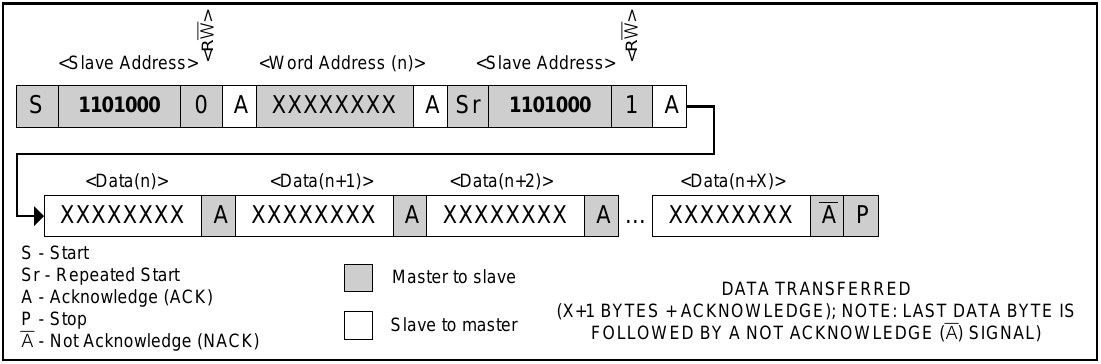
\includegraphics[scale=0.35]{images/ds1307-read-reg.png}
    \caption{DS1307 Read Starting From Specified Register}
  \end{figure}
  \vspace*{-5mm}
  \begin{itemize}
    \item If the register pointer is not written to before the initiation of a
          read mode, the first address that is read is the last one stored in
          the register pointer
    \item The register pointer automatically increments after each byte are read
  \end{itemize}
\end{frame}

\begin{frame}
  \frametitle{RTC Registers}
  \begin{figure}
    \centering
    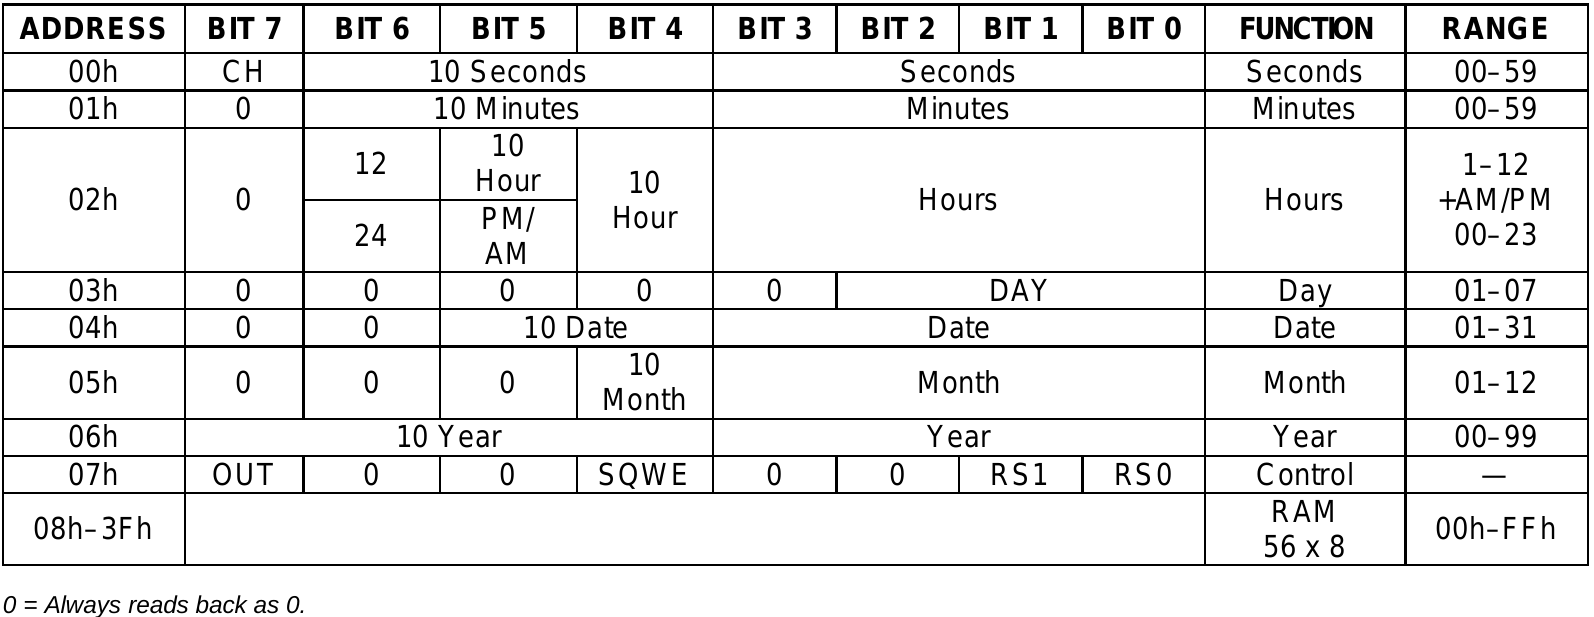
\includegraphics[scale=0.3]{images/rtc-registers.png}
    \caption{DS1307 I2C Registers}
  \end{figure}
\end{frame}

\begin{frame}
  \frametitle{RTC Read From Register (cont'd)}
  From DS1307 datasheet:
  \begin{itemize}
    \item ``The divider chain is reset whenever the seconds register is written. Write transfers
occur on the I2C acknowledge from the DS1307. Once the divider chain is reset,
to avoid rollover issues, the remaining time and date registers must be written within one second''
    \item ...So it's recommended to write all registers (time/date) in one transfer, starting from seconds register write
  \end{itemize}
\end{frame}

% ------------------------------------------------------------------------------

\section{Kernel Driver}

\subsection{I2C Kernel Subsystem}

\begin{frame}
  \frametitle{I2C IP-Core in SoC}
  \begin{figure}
    \centering
    \vspace*{-3mm}
    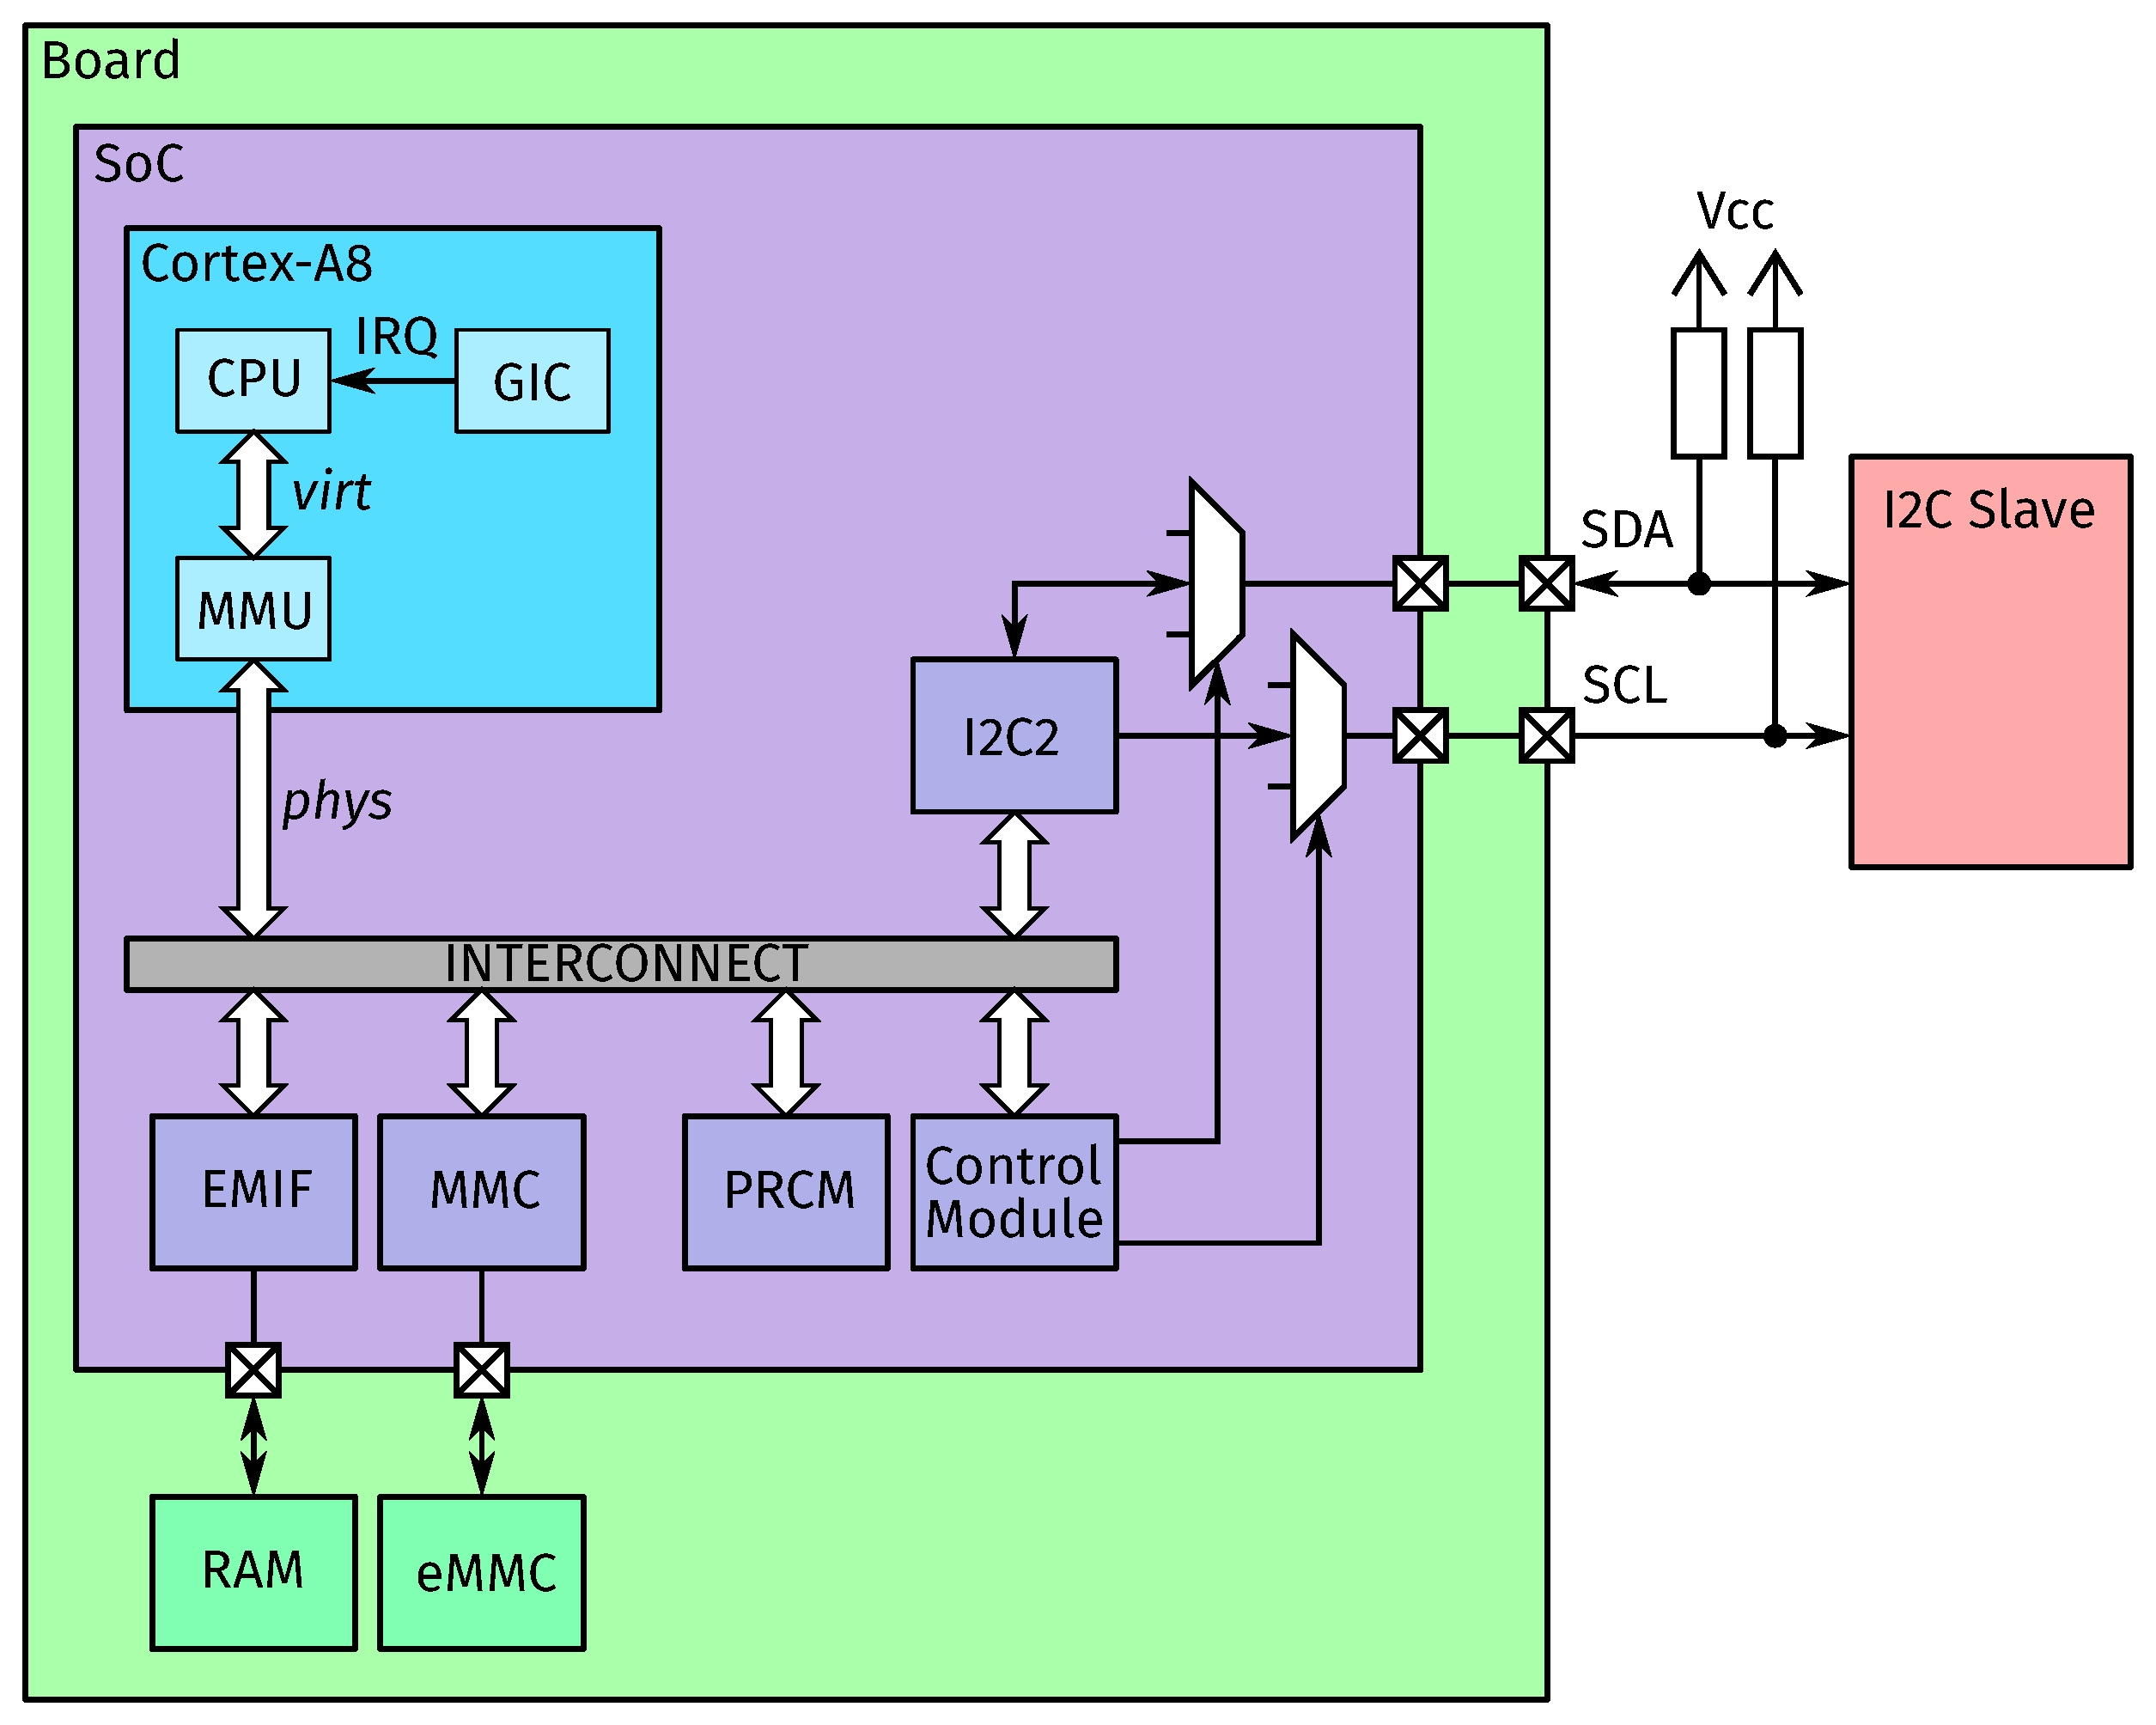
\includegraphics[scale=0.2]{images/architecture-i2c.pdf}
    \vspace*{-3mm}
    \caption{Integration of I2C Hardware Module in AM335x SoC}
  \end{figure}
  \vspace*{-12mm}
\end{frame}

\begin{frame}
  \frametitle{I2C Subsystem Driver Architecture}
  \begin{columns}
    \column{0.4\textwidth}
      There are 3 driver layers:
      \begin{itemize}
        \item \textbf{Adapter}: I2C controller driver; usually incudes algorithm
        \item \textbf{i2c-core}: I2C/SMBus protocols implementation;
              device/driver match
        \item \textbf{Client}: Driver for particular device on I2C
      \end{itemize}
    \column{0.6\textwidth}
      \vspace*{-3mm}
      \begin{figure}
        \centering
        \includegraphics[scale=0.35]{images/i2c-layers.pdf}
      \end{figure}
      \vspace*{-9mm}
  \end{columns}
\end{frame}

\begin{frame}
  \frametitle{I2C Call Chain}
  \begin{figure}
    \centering
    \includegraphics[scale=0.4]{images/i2c-call-chain.pdf}
  \end{figure}
  \begin{enumerate}
    \item User space application reads from character device file
    \item Device driver calls I2C API function (from I2C core)
    \item I2C core calls transfer callback from registered algorithm
    \item Callback leads to adapter driver transfer function
    \item Adapter driver initiates physical transfer on I2C bus
    \item Data is obtained from device and passed back to user space
  \end{enumerate}
  \vspace*{-7mm}
\end{frame}

\begin{frame}[containsverbatim]
  \frametitle{I2C Adapter Driver}
  \begin{itemize}
    \item Makes it possible to write \alert{platform-independent} drivers
    \item Driver: \texttt{drivers/i2c/busses/i2c-omap.c}
    \item Bindings: \texttt{Documentation/devicetree/bindings/i2c/i2c-omap.txt}
    \item Enabled in: \texttt{arch/arm/boot/dts/am33xx.dtsi}:
  \end{itemize}
  \begin{lstlisting}
/ {
	ocp {
		i2c2: i2c@4819c000 {
			compatible = "ti,omap4-i2c";
			#address-cells = <1>;
			#size-cells = <0>;
			ti,hwmods = "i2c3";
			reg = <0x4819c000 0x1000>;
			interrupts = <30>;
			status = "disabled";
		};
	};
};
  \end{lstlisting}
  \vspace*{-12mm}
\end{frame}

\begin{frame}
  \frametitle{Driver Model is Recursive (PC use-case)}
  \vspace*{-3mm}
  \begin{figure}
    \centering
    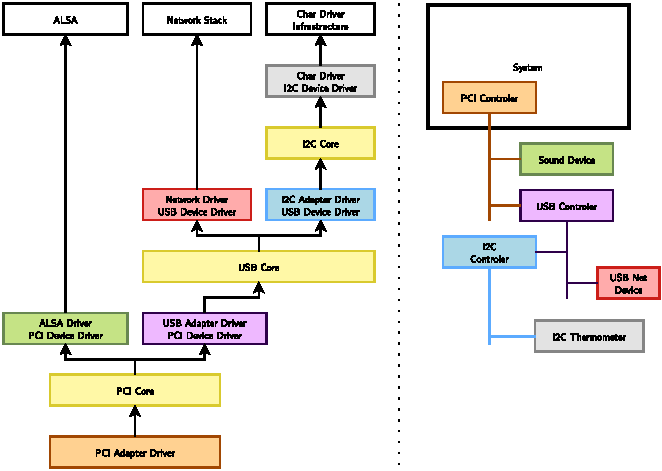
\includegraphics[scale=0.95]{images/driver-model.pdf}
  \end{figure}
  \vspace*{-12mm}
\end{frame}

\begin{frame}[standout]
  Take Five
\end{frame}

% ------------------------------------------------------------------------------

\subsection{Kernel APIs}

\begin{frame}
  \frametitle{Kernel Frameworks}
  \begin{itemize}
    \item Buses-centric API (for clients):
      \begin{itemize}
        \item I2C: \texttt{linux/i2c.h}
        \item SPI: \texttt{linux/spi/spi.h}
        \item USB: \texttt{linux/usb.h}
      \end{itemize}
    \item Device function centric frameworks:
      \begin{itemize}
        \item IIO (sensors, ADC, DAC): \texttt{linux/iio/iio.h}
        \item RTC: \texttt{linux/rtc.h}
        \item input\_dev: \texttt{linux/input.h}
      \end{itemize}
    \item Helpers:
      \begin{itemize}
        \item regmap: \texttt{linux/regmap.h}
        \item MFD: \texttt{linux/mfd/core.h}
      \end{itemize}
  \end{itemize}
\end{frame}

\begin{frame}[containsverbatim]
  \frametitle{Plain I2C Communication}
  \begin{lstlisting}[style=c]
int i2c_master_send(struct i2c_client *client, const char *buf, int count);
int i2c_master_recv(struct i2c_client *client, char *buf, int count);
  \end{lstlisting}
  \begin{itemize}
    \item These routines read and write some bytes from/to a client
    \item The client contains the i2c address, so you do not have to include it
    \item The second parameter contains the bytes to read/write
    \item The third the number of bytes to read/write
          (must be less than the length of the buffer, also should be
          less than 64k since msg.len is \texttt{u16})
    \item Returned is the actual number of bytes read/written
  \end{itemize}
\end{frame}

\begin{frame}[containsverbatim]
  \frametitle{Plain I2C Communication (cont'd)}
  \begin{lstlisting}[style=c]
int i2c_transfer(struct i2c_adapter *adap, struct i2c_msg *msg, int num);
  \end{lstlisting}
  \begin{itemize}
    \item This sends a series of messages
    \item Each message can be a read or write, and they can be mixed in any way
    \item The transactions are combined: no stop bit is sent between transaction
    \item The \texttt{i2c\_msg} structure contains for each message:
      \begin{itemize}
        \item the client address
        \item the number of bytes of the message
        \item and the message data itself
      \end{itemize}
  \end{itemize}
\end{frame}

\begin{frame}
  \frametitle{SMBus Communication}
  \begin{itemize}
    \item SMBus = System Management Bus
    \item SMBus protocol is a subset from the I2C protocol
    \item Many devices use only the same subset
    \item If you write a driver for some I2C device, please try to use the SMBus
          commands if at all possible
    \item This makes it possible to use the device driver on both SMBus adapters
          and I2C adapters
    \item (the SMBus command set is automatically translated to I2C on I2C
          adapters, but plain I2C commands can not be handled at all on most
          pure SMBus adapters)
  \end{itemize}
\end{frame}

\begin{frame}[containsverbatim]
  \frametitle{SMBus Communication (cont'd)}
  \vspace*{-5mm}
  \begin{lstlisting}[style=c]
s32 i2c_smbus_read_byte(struct i2c_client *client);
s32 i2c_smbus_write_byte(struct i2c_client *client, u8 value);
s32 i2c_smbus_read_byte_data(struct i2c_client *client, u8 command);
s32 i2c_smbus_write_byte_data(struct i2c_client *client, u8 command, u8 value);
s32 i2c_smbus_read_word_data(struct i2c_client *client, u8 command);
s32 i2c_smbus_write_word_data(struct i2c_client *client, u8 command, u16 value);
s32 i2c_smbus_read_block_data(struct i2c_client *client, u8 command, u8 *values);
s32 i2c_smbus_write_block_data(struct i2c_client *client, u8 command, u8 length, const u8 *values);
s32 i2c_smbus_read_i2c_block_data(struct i2c_client *client, u8 command, u8 length, u8 *values);
s32 i2c_smbus_write_i2c_block_data(struct i2c_client *client, u8 command, u8 length,
				   const u8 *values);
  \end{lstlisting}
  \begin{itemize}
    \item All these transactions return a negative errno value on failure
    \item The `write' transactions return 0 on success
    \item The `read' transactions return the read value, except for block
          transactions, which return the number of values read
    \item The block buffers need not be longer than 32 bytes
  \end{itemize}
  \vspace*{-5mm}
\end{frame}

\begin{frame}
  \frametitle{regmap}
  \begin{itemize}
    \item regmap = Register Map
    \item Register I/O for I2C and SPI
    \item We can use it instead of discussed I2C API
    \item Eliminates redundancy between drivers
    \item Can cache registers
    \item Can handle locking
    \item Can handle endianness conversion
  \end{itemize}
\end{frame}

\begin{frame}[containsverbatim]
  \frametitle{regmap API}
  \begin{lstlisting}[style=c]
#include <linux/regmap.h>

struct regmap_config {
	int reg_bits;			/* number of bits in register addr */
	int val_bits;			/* number of bits in register value */
	unsigned int max_register;	/* maximum valid register address */
	...
};

struct regmap *devm_regmap_init_i2c(struct i2c_client *i2c,
				    struct regmap_config *config);
int regmap_read(struct regmap *map, unsigned int reg, unsigned int *val);
int regmap_write(struct regmap *map, unsigned int reg, unsigned int val);
int regmap_bulk_read(struct regmap *map, unsigned int reg, void *val,
		     size_t val_count);
int regmap_bulk_write(struct regmap *map, unsigned int reg, const void *val,
int regmap_update_bits(struct regmap *map, unsigned int reg,
		       unsigned int mask, unsigned int val);
  \end{lstlisting}
\end{frame}

\begin{frame}
  \frametitle{RTC in kernel}
  \begin{itemize}
    \item RTC framework creates character device: \\
          \texttt{/dev/rtc0}, \texttt{/dev/rtc1}, etc; \\
          We can \texttt{read()} and \texttt{ioctl()} that file
    \item RTC framework also creates sysfs nodes in: \\
          \texttt{/sys/class/rtc/rtcX/} \\
          We can use \texttt{wakealarm} node to set alarm
    \item There are existing user-space tools in Linux:
      \begin{itemize}
        \item \texttt{hwclock}
        \item \texttt{rtcwake}
        \item \texttt{date}
      \end{itemize}
    \item Our device doesn't have alarm interrupt
  \end{itemize}
\end{frame}

\begin{frame}[containsverbatim]
  \frametitle{RTC API}
  \begin{lstlisting}[style=c]
#include <linux/rtc.h>

struct rtc_class_ops {
	int (*read_time)(struct device *, struct rtc_time *);
	int (*set_time)(struct device *, struct rtc_time *);
	int (*read_alarm)(struct device *, struct rtc_wkalrm *);
	int (*set_alarm)(struct device *, struct rtc_wkalrm *);
	int (*alarm_irq_enable)(struct device *, unsigned int enabled);
	`...`
};

struct rtc_device *devm_rtc_allocate_device(struct device *dev);

rtc->uie_unsupported = 1; /* no IRQ line = no Update Interrupt Enable */
rtc->ops = (struct rtc_class_ops)`...`;

int rtc_register_device(struct rtc_device *rtc);
  \end{lstlisting}
\end{frame}

\begin{frame}[containsverbatim]
  \frametitle{RTC API (cont'd)}
  \begin{lstlisting}[style=c]
/* If device has alarm interrupt line (DS1307 doesn't) */
void rtc_update_irq(struct rtc_device *rtc, unsigned long num,
		    unsigned long events);

`\textbf{Helper functions:}`
int rtc_year_days(unsigned int day, unsigned int month, unsigned int year);
int rtc_valid_tm(struct rtc_time *tm);
time64_t rtc_tm_to_time64(struct rtc_time *tm);
`...`
  \end{lstlisting}
  There is also \texttt{nvmem} API, but we won't cover it here.
\end{frame}

\begin{frame}[containsverbatim]
  \frametitle{BCD Format}

  \begin{itemize}
    \item BCD = binary-coded decimal
    \item Each of the two nibbles of each byte represent a decimal digit
  \end{itemize}

  \begin{figure}
    \centering
    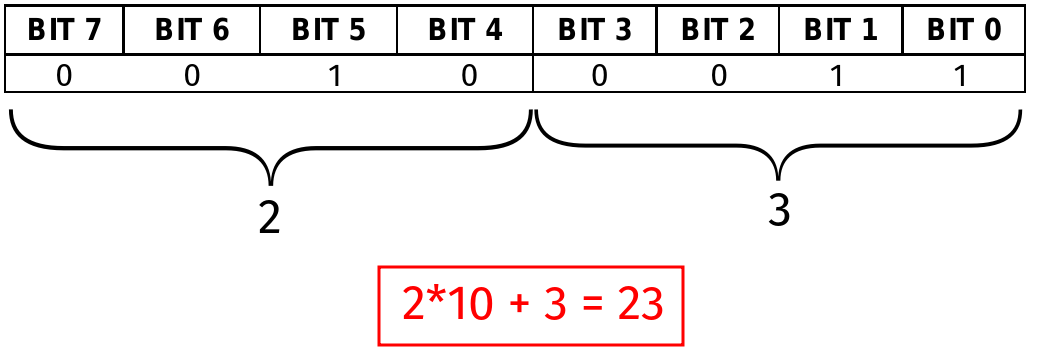
\includegraphics[scale=0.3]{images/bcd.png}
  \end{figure}

BCD helper functions:
  \begin{lstlisting}[style=c]
#include <linux/bcd.h>

unsigned bcd2bin(unsigned char val); /* decode BCD value to dec value */
unsigned char bin2bcd(unsigned val); /* encode dec value to BCD value */
  \end{lstlisting}
  \vspace*{-5mm}
\end{frame}

\begin{frame}
  \frametitle{Bit-banged I2C}
  ``Bit-banging'' is GPIO emulation of some protocol.
  \begin{itemize}
    \item Can be useful on cheap boards without I2C controllers
    \item ...or if there is no unused I2C addresses left on bus
    \item There is already implemented bit-banged I2C driver: \\
    \texttt{Documentation/devicetree/bindings/i2c/i2c-gpio.txt}
    \item There are more ready to use GPIO drivers; for details see: \\
          \texttt{Documentation/driver-api/gpio/drivers-on-gpio.rst}
  \end{itemize}
\end{frame}

\begin{frame}[containsverbatim]
  \frametitle{Linux Turns 28! \textit{(25 Aug)}}
  \begin{columns}
    \column{0.5\textwidth}
      \begin{itemize}
        \item A lot of frameworks already exist
        \item Check out \texttt{Documentation/}
        \item \sout{Doxygen} kernel-doc comments
        \item Linux code base is a good source of examples
        \item \texttt{git grep} is useful to find references:
          \begin{lstlisting}[language=bash]
`\$` git grep -l --all-match -e devm_regmap \
           -e devm_rtc -- drivers/
`\$` git grep -n -e _i2c_init --and \( -e module \
           -e initcall \) -- '*.[ch]'
          \end{lstlisting}
      \end{itemize}
    \column{0.5\textwidth}
      \begin{figure}
        \centering
        
\includegraphics[scale=0.4]{images/linux-bday.png}
      \end{figure}
      \vspace*{-6mm}
  \end{columns}
\end{frame}

% ------------------------------------------------------------------------------

\subsection{RTC Driver Implementation}

\begin{frame}[standout]
  RTC Driver Implementation
\end{frame}

\begin{frame}[containsverbatim]
  \frametitle{Device Tree Definition}
  \begin{lstlisting}[caption=Device Tree definition for our driver]
&i2c2 {
	ds1307x: ds1307x@68 {
		compatible = "dallas,ds1307x";
		reg = <0x68>;
	};
};
  \end{lstlisting}
Note that:
  \begin{itemize}
    \item \texttt{i2c2\_pins} are already muxed
          (\texttt{PIN\_INPUT\_PULLUP | MUX\_MODE3})
    \item \texttt{i2c2.status} is \texttt{okay}
    \item Our driver will be bound on \texttt{insmod}
  \end{itemize}
\end{frame}

\begin{frame}[containsverbatim]
  \frametitle{I2C Driver: Init}
  \begin{lstlisting}[caption=Initialization of I2C driver, style=c]
static struct i2c_driver ds1307x_driver = {
	.driver = {
		.name		= "ds1307x",
		.of_match_table	= ds1307x_of_match,
	},
	.probe		= ds1307x_probe,
	.remove		= ds1307x_remove,
	.id_table	= ds1307x_id,
};

module_i2c_driver(ds1307x_driver);
  \end{lstlisting}
\end{frame}

\begin{frame}[containsverbatim]
  \frametitle{I2C Driver: Device Tables}
  \begin{lstlisting}[caption=Device Tables used in our driver, style=c]
static const struct i2c_device_id ds1307x_id[] = {
	{ "ds1307x" },
	{ },
};
MODULE_DEVICE_TABLE(i2c, ds1307x_id);

static const struct of_device_id ds1307x_of_match[] = {
	{ .compatible = "dallas,ds1307x" }, /* ds1307 already exists */
	{ }
};
MODULE_DEVICE_TABLE(of, ds1307x_of_match);
  \end{lstlisting}
\end{frame}

\begin{frame}[containsverbatim]
  \frametitle{I2C Driver: Probe and remove}
  \begin{lstlisting}[caption=Probe and remove functions in our driver, style=c]
#include <linux/module.h>
#include <linux/i2c.h>

static int ds1307x_probe(struct i2c_client *client,
			 const struct i2c_device_id *id)
{
	/* TODO */
	return 0;
}

static int ds1307x_remove(struct i2c_client *client)
{
	/* TODO */
	return 0;
}
  \end{lstlisting}
\end{frame}

\begin{frame}[containsverbatim]
  \frametitle{Raw API Example}
  \vspace*{-8mm}
  \begin{lstlisting}[caption=Example of raw I2C API usage, style=c]
	int ret;
	u8 reg = 0x01;	/* I2C register */
	u8 buf;		/* where to read */
	u8 len = 1;	/* bytes to read */
	struct i2c_msg msg[2] = {
		{
			.addr = client->addr,
			.len = 1,
			.buf = &reg,
		},
		{
			.addr = client->addr,
			.flags = I2C_M_RD,	/* read */
			.len = len,
			.buf = &buf,
		}
	};

	ret = i2c_transfer(client->adapter, msg, 2);
	if (ret < 0)
		return ret;

	pr_info("### read data = %#x\n", buf);
  \end{lstlisting}
  \vspace*{-12mm}
\end{frame}

\begin{frame}[containsverbatim]
  \frametitle{SMBus API Example}
  \begin{lstlisting}[caption=Example of SMBus API usage, style=c]
	s32 data;

	data = i2c_smbus_read_byte_data(client, 0x01); /* minutes */
	pr_info("### read data = %#x\n", data);
  \end{lstlisting}
\end{frame}

\begin{frame}[containsverbatim]
  \frametitle{Address Conflicts}
  \begin{itemize}
    \item Be aware of possible I2C address conflicts on the same bus!
    \item On \texttt{insmod} you can see something like this:
  \end{itemize}

  \vspace*{-5mm}
  \begin{lstlisting}[caption=Example of conflict on bus,language=]
i2c i2c-2: Failed to register i2c client ds1307 at 0x68 (`\textbf{-16}`)
i2c i2c-2: of_i2c: Failure registering /ocp/i2c@4819c000/ds1307@68
i2c i2c-2: Failed to create I2C device for /ocp/i2c@4819c000/ds1307@68
  \end{lstlisting}

Where 16 is \texttt{EBUSY}.

  \begin{lstlisting}[caption=No conflict]
rtc-ds1307 2-0068: SET TIME!
rtc-ds1307 2-0068: registered as rtc1
  \end{lstlisting}
\end{frame}

\begin{frame}[containsverbatim]
  \frametitle{Userspace Tools}
  Let's check if our device is visible on bus:
  \begin{lstlisting}[language=bash]
`\#` i2cdetect -r 2 -y

     0  1  2  3  4  5  6  7  8  9  a  b  c  d  e  f
00:          -- -- -- -- -- -- -- -- -- -- -- -- --
10: -- -- -- -- -- -- -- -- -- -- -- -- -- -- -- --
20: -- -- -- -- -- -- -- -- -- -- -- -- -- -- -- --
30: -- -- -- -- -- -- -- -- -- -- -- -- -- -- -- --
40: -- -- -- -- -- -- -- -- -- -- -- -- -- -- -- --
50: 50 -- -- -- -- -- -- -- -- -- -- -- -- -- -- --
60: -- -- -- -- -- -- -- -- 68 -- -- -- -- -- -- --
70: -- -- -- -- -- -- -- --
  \end{lstlisting}

  After \texttt{insmod} we'll see \texttt{UU} instead \texttt{68}
  (means it's used).\\
  We can also use \texttt{i2cdump}, \texttt{i2cget} and \texttt{i2cset} tools:
  \begin{lstlisting}[language=bash]
`\#` i2cget -y 2 0x68 0x01

0x49
  \end{lstlisting}
  \vspace*{-2mm}
\end{frame}

\begin{frame}[containsverbatim]
  Once driver is implemented, we can use it for keeping the system time:
  \frametitle{Userspace Tools (cont'd)}
  \begin{lstlisting}[language=bash]
`\textbf{Set system time:}`
`\#` date -s "2018-08-28 11:30:00"

`\textbf{Write system time to our RTC:}`
`\#` hwclock -w -f /dev/rtc1

`\textbf{Read time from our RTC:}`
`\#` hwclock -r -f /dev/rtc1

`\textbf{Set system time from our RTC:}`
`\#` hwclock -s -f /dev/rtc1

`\textbf{Show system time:}`
`\#` date
  \end{lstlisting}
\end{frame}

% ------------------------------------------------------------------------------

\section{Assignments}

\begin{frame}
  \frametitle{Assignment 1 (basic)}
  \underline{Implement Proof-of-Concept driver}:
  \begin{itemize}
    \item Connect RTC module to your BBB
    \item Check with \texttt{i2cdetect} tool it's visible on bus
    \item Write Device Tree definition for your driver (use \texttt{"ds1307x"}
          as compatible string)
    \item Write I2C driver boilerplate; make sure that \texttt{probe()} is
          called
    \item Try to read from some I2C register; make sure it's the same value as
          \texttt{i2cget} tool reports
    \item Next documents will help you to implement the driver:
    \begin{itemize}
      \item \href{https://datasheets.maximintegrated.com/en/ds/DS1307.pdf}
                 {DS1307 Datasheet}
      \item \href {https://www.nxp.com/docs/en/user-guide/UM10204.pdf}
                  {I2C Specification}
      \item \href {https://www.kernel.org/doc/html/v4.19/}
                  {Kernel API Documentation} (look for I2C API)
    \end{itemize}
  \end{itemize}
\end{frame}

\begin{frame}
  \frametitle{Assignment 2 (advanced)}
  \underline{Implement productizable driver}:
  \begin{itemize}
    \item Implement reading/writing registers via regmap
    \item Implement RTC using RTC kernel API
    \item Set your RTC using \texttt{hwclock} tool; make sure it works
    \item Test if it's consistent between power-off / power-on
    \begin{itemize}
      \item Module's battery might be discharged; in that case it won't store
            your data after power-off
    \end{itemize}
    \item \textbf{Hint}: If in troubles, use existing drivers as
          examples/templates
  \end{itemize}
\end{frame}

\begin{frame}
  \frametitle{References}
  \begin{thebibliography}{}
  \setbeamertemplate{bibliography item}[book]
  \bibitem{LDDD2017}
    John Madieu.
    \newblock \emph{Linux Device Drivers Development}.
  \bibitem{ELSDD2006}
    P. Raghavan, Amol Lad, Sriram Neelakandan.
    \newblock \emph{Embedded Linux System Design and Development}.
  \setbeamertemplate{bibliography item}[article]
  \bibitem{I2C} \texttt{Documentation/i2c/writing-clients}
  \end{thebibliography}
\end{frame}

\begin{frame}[standout]
  Thank you!
\end{frame}

% ------------------------------------------------------------------------------

\end{document}
